% Dit werk is gelicenseerd onder de licentie Creative Commons Naamsvermelding-GelijkDelen 4.0 Internationaal. Ga naar http://creativecommons.org/licenses/by-sa/4.0/ om een kopie van de licentie te kunnen lezen.
\chapter{Tabellen en grafieken}
\label{sec:Tabellen en grafieken}

\makeatletter
\setlength{\@fptop}{0pt}
\makeatother
\captionsetup{justification=justified,singlelinecheck=false}

\captionof{table}{Verliescoëfficiënt bij stroming door een cirkelvormige bocht van 90\deg}
\begin{tabular}[t]{p{12cm} p{5cm}}
	\begin{tabular}{l c c c c c}
		$r/D$        & 1    & 2    & 4    & 6    & 10   \\
		\hline
		$\zeta$ glad & 0.21 & 0.14 & 0.11 & 0.09 & 0.11 \\
		$\zeta$ ruw  & 0.51 & 0.30 & 0.23 & 0.18 & 0.20 \\
	\end{tabular}
	&
	\smash{\raisebox{-0.5\height}{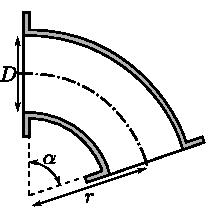
\includegraphics{fig/appendix/Bocht}}}
\end{tabular}

\captionof{table}{Correctiefactor voor cirkelvormige bochten met andere hoeken}
\begin{tabular}[t]{p{12cm} p{5cm}}
	\begin{tabular}{l c c c c c c}
		$\alpha$ & 30\deg & 60\deg & 90\deg & 120\deg & 150\deg & 180\deg   \\ 
		\hline
		$k$    & 0.4    & 0.7    & 1      & 1.25    & 1.5     & 1.7 \\
	\end{tabular}
	&
\end{tabular}

\captionof{table}{Verliescoëfficiënt voor een plotse verwijding}
\begin{tabular}[t]{p{12cm} p{5cm}}
	\begin{tabular}{l c c c c c c c c c}
		$D_2/D_1$ & 1.0 & 1.2 & 1.4 & 1.6 & 1.8 & 2.0 & 3.0 & 5.0 & $\infty$ \\ 
		\hline
		$\zeta$    & 0.00    & 0.09    & 0.24      & 0.37    & 0.48     & 0.56 & 0.79 & 0.92 & 1.00 \\
	\end{tabular}
	&
	\vfill
	\smash{\raisebox{-0.5\height}{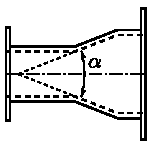
\includegraphics{fig/appendix/Verwijding}}}
\end{tabular}
\vspace{1cm}

\captionof{table}{Correctiefactor voor geleidelijke verwijding}
\begin{tabular}[t]{p{12cm} p{5cm}}
	\begin{tabular}{l c c c c c c c c c c}
		$\alpha$ & 6\deg & 10\deg & 15\deg & 20\deg & 30\deg & 40\deg & 50\deg & 60\deg & 70\deg & 90\deg \\ 
		\hline
		$k$    & 0.14    & 0.20    & 0.30      & 0.40    & 0.70     & 0.90 & 1.00 & 1.10 & 1.10 & 1.00 \\
	\end{tabular}
	&
	\vfill
	\smash{\raisebox{-0.5\height}{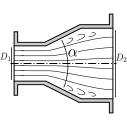
\includegraphics{fig/appendix/Gelijdelijke_verwijding}}}
\end{tabular}
\vspace{1cm}

\captionof{table}{Verliescoëfficiënt bij stroming door een plotse vernauwing}
\begin{tabular}[t]{p{12cm} p{5cm}}
	\begin{tabular}{l c c c c c c c c c}
		$D_1/D_2$ & 4.0 & 3.5 & 3.0 & 2.5 & 2.0 & 1.5 & 1.3 & 1.1 & 1.0   \\ 
		\hline
		$\zeta$    & 0.45    & 0.43    & 0.42      & 0.40    & 0.37     & 0.28 & 0.20 & 0.01 & 0 \\
	\end{tabular}
	&
	\vfill
	\smash{\raisebox{-0.5\height}{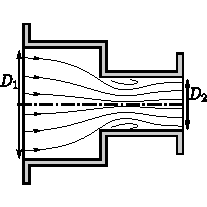
\includegraphics{fig/appendix/Vernauwing}}}
\end{tabular}

\begin{figure}[ht]
	\caption{Moody diagram}
	\label{fig:Moody diagram}
	\centering
	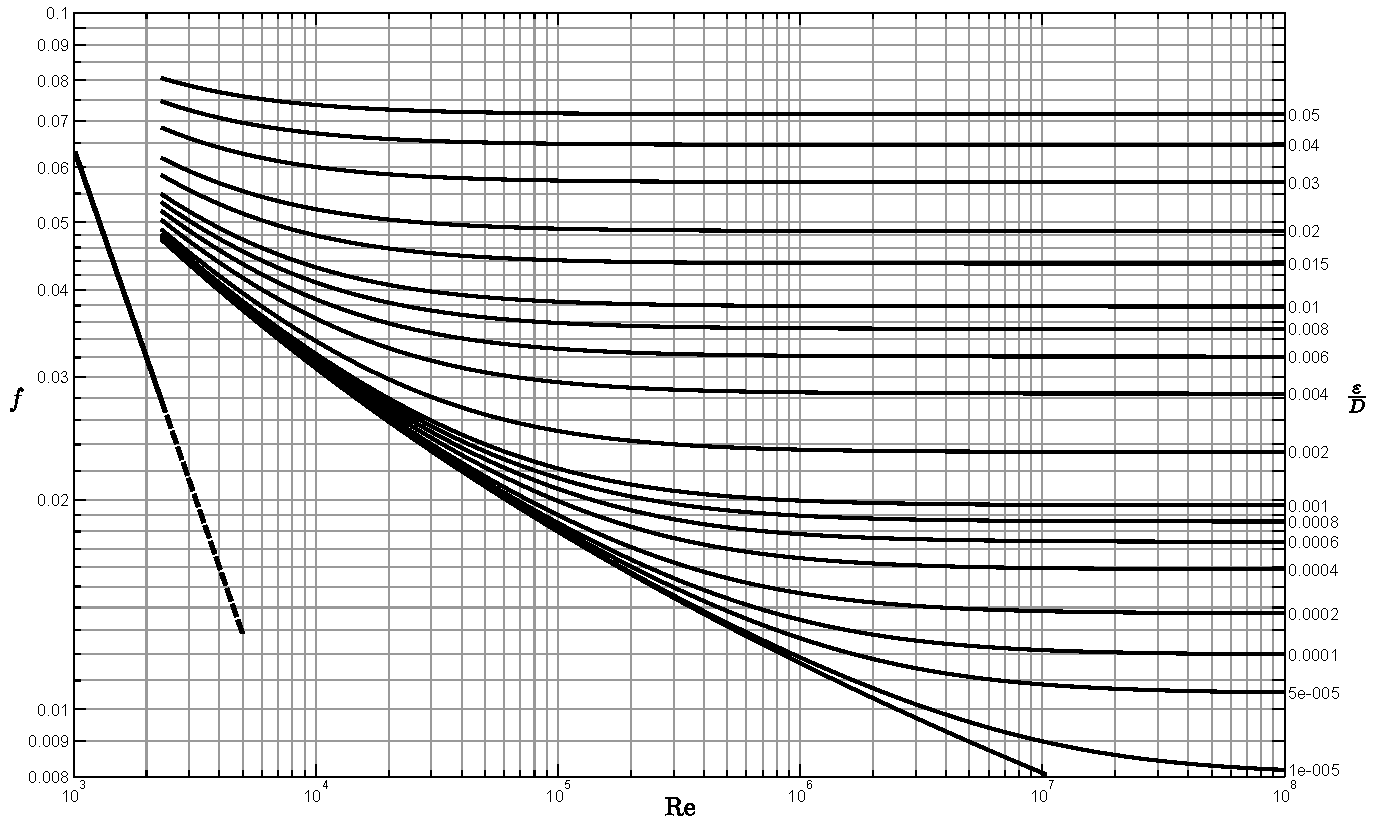
\includegraphics[width=22cm, angle=270]{fig/stroming_in_leidingen/Moody_diagram.pdf}
\end{figure}